Nous avons utilisé Git dès le début du projet. Comme nous l'avions presque tous déja utilisé, son utilisation était évidente, sachant qu'en plus, c'est l'un des gestionnaire de code le plus performant.
Nous avons installé un depôt sur le Git du Sif. Nous avons utilisé une branche Master, qui devait contenir uniquement du code compilable, et après, chaque fonctionnalités à été développé sur une branche différentes.
Nous utilisons également Gitg, pour avoir une meilleure vue de l'état de notre dêpot. Voir ~\ref{Gitg} page~\pageref{Gitg}.
\begin{figure}[h]
\caption{\label{Gitg} Capture de Gitg}
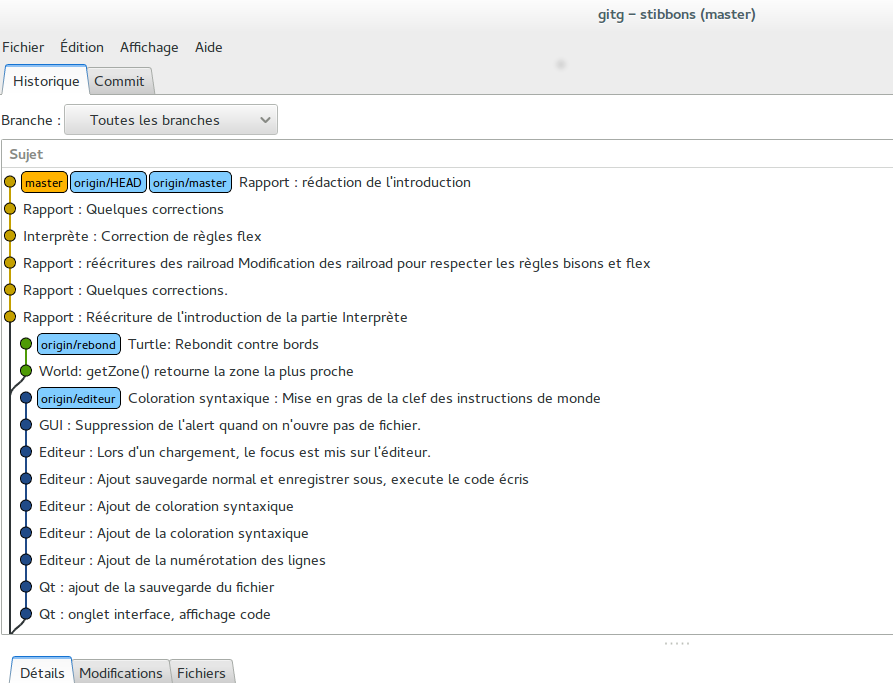
\includegraphics[scale=0.35]{doc/report/gitbranche.png}
\end{figure}
